%----------------------------------------------------------------------------------------
%    PACKAGES AND THEMES
%----------------------------------------------------------------------------------------

\documentclass[aspectratio=169,xcolor=dvipsnames]{beamer}
\usepackage[spanish,es-tabla,es-nodecimaldot]{babel}

\usetheme{SimpleDarkBlue}

\usepackage{hyperref}
\usepackage{graphicx} % Allows including images
\usepackage{booktabs} % Allows the use of \toprule, \midrule and \bottomrule in tables
\usepackage{physics}
\usepackage{tikz}
%#########################################################
%#########  Modificar caption #############################
%#######################################################

\usepackage[font=tiny, justification=centering]{caption}  % Configura las captions



\newcommand{\parentesis}[1]{\left( #1  \right)}
\newcommand{\parciales}[2]{\frac{\partial #1}{\partial #2}}
\newcommand{\pparciales}[2]{\parentesis{\parciales{#1}{#2}}}
\newcommand{\ccorchetes}[1]{\left[ #1  \right]}
\newcommand{\D}{\mathrm{d}}
\newcommand{\derivadas}[2]{\frac{\D #1}{\D #2}}

\newcommand{\tquad}{\quad \quad \quad}
%\newcommand{\vnabla}{\vec{\nabla}}

\newcommand{\Ocal}{\mathcal{O}}
\newcommand{\Jcal}{\mathcal{J}}
\newcommand{\Mcal}{\mathcal{M}}
\newcommand{\Fcal}{\mathcal{F}}
\newcommand{\Hcal}{\mathcal{H}}
\newcommand{\Ecal}{\mathcal{E}}
\newcommand{\Ncal}{\mathcal{N}}

\newcommand{\cmm}{\text{cm}^{-1}}
\newcommand{\fcc}{\textit{fcc}}
\newcommand{\bcc}{\textit{bcc}}
\renewcommand{\sc}{\textit{sc}}
\newcommand{\hcp}{\textit{hcp}}


\newcommand{\PZB}{\text{{\tiny PZB}}}
\newcommand{\gap}{\text{{\tiny gap}}}
\newcommand{\SZB}{\text{{\tiny SZB}}}
\newcommand{\inicial}{\text{{\tiny inicial}}}
\newcommand{\final}{\text{{\tiny final}}}
\newcommand{\atomico}{\text{{\tiny atómico}}}

\newcommand{\arctanh}{\text{{arctanh}}}



\newcommand{\Namas}{\text{Na}^+}
\newcommand{\Clmenos}{\text{Cl}^-}

\newcommand{\cm}{\text{cm}}
\newcommand{\eV}{\text{eV}}

\newcommand{\arr}{\text{arr}}
\newcommand{\diff}{\text{diff}}

\newcommand{\er}{$^{\text{er}}$}
\newcommand{\cte}{\text{cte}}


% Comandos vectoriales

\newcommand{\an}{\mathbf{a}}
\newcommand{\bn}{\mathbf{b}}
\newcommand{\dn}{\mathbf{d}}
\newcommand{\fn}{\mathbf{f}}
\newcommand{\jn}{\mathbf{j}}
\newcommand{\kn}{\mathbf{k}}
\newcommand{\pn}{\mathbf{p}}
\newcommand{\qn}{\mathbf{q}}
\newcommand{\rn}{\mathbf{r}}
\newcommand{\sn}{\mathbf{s}}
\newcommand{\un}{\mathbf{u}}
\newcommand{\vn}{\mathbf{v}}
\newcommand{\xn}{\mathbf{x}}
\newcommand{\wn}{\mathbf{w}}
\newcommand{\yn}{\mathbf{y}}
\newcommand{\qndot}{\dot{\qn}}

\newcommand{\alphan}{\boldsymbol{\alpha}}
\newcommand{\sigman}{\boldsymbol{\sigma}}
\newcommand{\pin}{\boldsymbol{\pi}}
\newcommand{\rhon}{\boldsymbol{\rho}}
\newcommand{\epsilonn}{\boldsymbol{\epsilon}}
\newcommand{\omegan}{\boldsymbol{\omega}}
\newcommand{\mun}{\boldsymbol{\mu}}



\newcommand{\An}{\mathbf{A}}
\newcommand{\Bn}{\mathbf{B}}
\newcommand{\En}{\mathbf{E}}
\newcommand{\Fn}{\mathbf{F}}
\newcommand{\Jn}{\mathbf{J}}
\newcommand{\Hn}{\mathbf{H}}
\newcommand{\Gn}{\mathbf{G}}
\newcommand{\Kn}{\mathbf{K}}
\newcommand{\Ln}{\mathbf{L}}
\newcommand{\Mn}{\mathbf{M}}
\newcommand{\Pn}{\mathbf{P}}
\newcommand{\Rn}{\mathbf{R}}
\newcommand{\Sn}{\mathbf{S}}
\newcommand{\Tn}{\mathbf{T}}
\newcommand{\In}{\mathbf{1}}
\newcommand{\Encal}{\boldsymbol{\mathcal{E}}}

\newcommand{\hnn}{\hat{\mathbf{n}}}
\newcommand{\hnr}{\hat{\mathbf{r}}}
\newcommand{\hnz}{\hat{\mathbf{z}}}
\newcommand{\hnv}{\hat{\mathbf{v}}}
\newcommand{\hnx}{\hat{\mathbf{x}}}
\newcommand{\hny}{\hat{\mathbf{y}}}
\newcommand{\hnu}{\hat{\mathbf{u}}}
\newcommand{\hnR}{\hat{\mathbf{R}}}
\newcommand{\hnp}{\hat{\mathbf{p}}}
\newcommand{\hnk}{\hat{\mathbf{k}}}
\newcommand{\hni}{\hat{\mathbf{i}}}
\newcommand{\hnj}{\hat{\mathbf{j}}}
\renewcommand{\hnk}{\hat{\mathbf{k}}}
%----------------------------------------------------------------------------------------
%    TITLE PAGE
%----------------------------------------------------------------------------------------

\title{Práctica de Electronica con ABACUS-Nanohub}
\subtitle{Union PN}

\author{Daniel Vázquez Lago}

%\institute
%{
%    Department of Computer Science and Information Engineering \\
%    National Taiwan University % Your institution for the title page
%}
\date{\today} % Date, can be changed to a custom date

%----------------------------------------------------------------------------------------
%    PRESENTATION SLIDES
%----------------------------------------------------------------------------------------

\begin{document}

\begin{frame}
    % Print the title page as the first slide
    \titlepage
\end{frame}

\begin{frame}{Overview}
    % Throughout your presentation, if you choose to use \section{} and \subsection{} commands, these will automatically be printed on this slide as an overview of your presentation
    \tableofcontents
\end{frame}

%------------------------------------------------
\section{Objetivos}
%------------------------------------------------
\begin{frame}{Objetivos}
    Nuestros objetivo es la comparación entre la teoría (ecuaciones del diodo ideal) y una simulación (proporcionada por ABACUS-Nanohub versión old) de las principales características de la unión PN para dos diodos diferentes con los siguientes valores:  

    \begin{table}
        \begin{tabular}{c|cccccc}
            & $m_p^*/m_e$ & $m_n^*/m_e$ & $\mu_p$  \tiny{[cm$^2$/(V$\cdot$s)]} & $\mu_n$ \tiny{[cm$^2$/(V$\cdot$s)]} & $T$ \tiny{[K]} & $E_g$ \tiny{[eV]} \\ \hline
            Diodo 1 & 0.81  & 1.19 & 460 & 1360 & 300 & 1.12  \\
            Diodo 2 & 0.81  & 1.19 & 460 & 1360 & 300 & 1.12  
        \end{tabular}
    \end{table}
    \begin{table}
        \begin{tabular}{c|cccccc}
             &  $\tau_n$ \tiny{[s]} & $\tau_p$ \tiny{[s]} & $x_{1n}$ \tiny{[$\mu$m]} & $x_{1p}$ \tiny{[$\mu$m]} & $N_D$ \tiny{[cm$^{-3}$]} & $N_A$  \tiny{[cm$^{-3}$]}\\ \hline
            Diodo 1  & $10^{-10}$ & $10^{-10}$ & 10 & 10 & $3.5 \cdot 10^{16}$ & $3.5 \cdot 10^{16}$ \\
            Diodo 2  & $10^{-10}$ & $10^{-10}$ & 10 & 10 & $3.5 \cdot 10^{17}$ & $3.5 \cdot 10^{16}$ 
        \end{tabular}
    \end{table}
    donde $m_p^*$ es la masa efectiva del hueco, $m_n^*$ la masa efectiva del electrón, $\mu_p$ la movilidad del hueco, $\mu_n$ la movilidad del electrón, $T$ la temperatura, $E_g$ la enerǵia del gap, $\tau_n$ la vida media del electrón, $\tau_p$ la movilidad del hueco, $x_{1n}$ el tamaño de la zona N, $x_{1p}$ el tamaño de la zona P, $N_D$ el dopado de dadores en la zona N y $N_A$ el dopado de aceptores en la zona P.
\end{frame}

\section{Modelo teórico: región de vaciamiento}

\begin{frame}{Marco teórico: zona de vaciamiento}
    La aproximación de la zona de vaciamiento consiste en consdierar que alrededor de la unión de los dopados $P$ y $N$  (denotada por $x=0$) existe una región delimitada por dos puntos ($-x_p$ y $x_n$) en los cuales tanto $n$ como $p$ son mucho más pequeños que los valores $N_D^+$ y $N_A^-$. Así en esta región existirá una densidad de carga no nula $\rho$ lo que generará un campo eléctrico y potencial eléctrico no nulo (en virtud de las ecuacioens de Maxwell). Las condiciones para poder realizar esta aproximación son:

    \begin{itemize}
        \item En las regiones $x<-x_p$ y $x_n<x$ llamadas regiones masivas $P$ y $N$ respectivamente, se verifica que \textit{todas las impurezas están ionizadas} y que \textit{la densidad de carga neta es cero}.
        \item En la región $-x_p<x<0$ tenemos que $n_p,p_p\ll N_A$ tal que $\rho=-qN_A^-$.
        \item En la región $0<x<x_n$ tenemos que $n_n,p_n\ll N_D$ tal que $\rho=qN_D^-$.
    \end{itemize} 
\end{frame}

\begin{frame}{Marco teórico: zona de vaciamiento}
    Llamamos al diodo 1 diodo simétrico y al diodo 2 diodo no simétrico. Los valores de $x_n$ y $x_p$ vienen dados por
    \begin{equation*}
        x_p = \ccorchetes{\frac{2K_S\varepsilon_0}{q} \frac{N_D}{N_A(N_A+N_D)}  V_{bi}}   \qquad 
        x_n = \ccorchetes{\frac{2K_S\varepsilon_0}{q} \frac{N_A}{N_D(N_A+N_D)}  V_{bi}}
    \end{equation*}
    \begin{equation*}
        V_{bi} = \frac{kT}{q} \ln \parentesis{\frac{N_AN_D}{n_i^2}} 
    \end{equation*}
    siendoo $V_{bi}$ el voltaje entre la región $P$ y $N$ en el equilibrio (no se le aplica voltaje al diodo). En la siguiente imagen representamos en gris la región de vaciamiento, separadas de las zonas masvias por $x_p$ y $x_n$:
    \begin{figure} 
        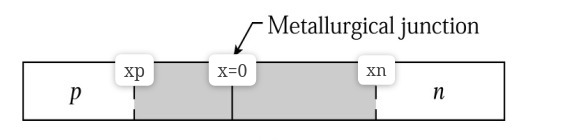
\includegraphics[width=0.5\linewidth]{Foto_Union.jpeg}
    \end{figure}
\end{frame}

%-------------------------------
\section{Modelo teórico: diodo ideal}

\begin{frame}{Marco teórico: diodo ideal}
    El modelo del diodo ideal nos permite obtener de manera analítica valores para las corrientes $J_N$ y $J_P$ a lo largo del dispositivo cuando aplicamos un voltaje $V_A$ externo entre el diodo $P$ y $N$, a través de las siguientes ecuaciones: 
    \begin{itemize}
        \item Podemos hacer la aproximación de la zona de vaciamiento.
        \item Estado estacionario. 
        \item No existe recombinación ni generación de portadores en la región de vaciamiento. 
        \item Bajo nivel de inyección en todo el dispositivo. 
        \item No hay degeneración. 
        \item Toda la tensión cae en las zona de vaciamiento. Contactos óhmicos perfectos y conductor perfecto en zonas masivas. 
        \item Las regiones masivas y la región de vacimineto están dopadas uniformemente.
        \item Los cuasi-niveles de Fermi son constantes en la zona de transición. 
    \end{itemize}
\end{frame}

\begin{frame}{Densidad de carga}
    La denisdad de carga $\rho$ viene dada por:
    \begin{equation*}
        \rho (x) = \left\lbrace \begin{array}{ll}
            - q N_A   & \ - x_p \leq x \leq 0 \\
            q N_D  & \ 0 \leq x \leq x_n \\
        \end{array} \right.
    \end{equation*}
    siendo cero en las zonas masivas. El campo eléctrico se calcula a partir de la ecuación de Maxwell
    \begin{equation*}
        \nabla \cdot \Ecal = \frac{\rho}{K_S \epsilon_0}
    \end{equation*}
\end{frame}


\begin{frame}{Campo y potencial eléctrico}
    El campo eléctrico viene dado por la siguiente ecuación: 
    \begin{equation*}
        \Ecal(x) = \left\lbrace \begin{array}{ll}
            - \frac{qN_A}{K_S\varepsilon_0} \parentesis{x_p - x}  & \ - x_p \leq x \leq 0 \\
            - \frac{qN_D}{K_S\varepsilon_0} \parentesis{x_n - x} & \ 0 \leq x \leq x_n \\
        \end{array} \right.
    \end{equation*}
    siendo 0 en las regiones masivas. El potencial elétrico viene dado por: 
    \begin{equation*}
        V_{J} = V_{bi} - V_A
    \end{equation*}
    \begin{equation*}
        V(x) = \left\lbrace \begin{array}{ll}
            0  & x \leq -x_p  \\
            \frac{qN_A}{2K_S\varepsilon_0} \parentesis{x_p + x}^2  & \ - x_p \leq x \leq 0 \\
            - \frac{qN_D}{2K_S\varepsilon_0} \parentesis{x_n - x}^2 + V_{J}  & \ 0 \leq x \leq x_n \\
            V_{J} & x_n \leq 0
        \end{array} \right.
    \end{equation*}
\end{frame}

\begin{frame}{Bandas de energía}
    En cálculo de las bandas de energía se realiza de la siguiente manera. Primero calculamos los valores para la zona P:  
    \begin{equation*}
        E_i|_P = kT \ln \parentesis{\frac{N_{A}}{n_i}} \qquad E_c |_P = E_i |_P + \frac{3kT}{4}\ln \parentesis{\frac{m_p^*}{m_n^*} } \qquad E_v|_P  =E_c|_P-E_g 
    \end{equation*}
    donde $|_{P}$ indica que se ha calculado en la región masiva P. Dado que las bandas deben verificar:

    \begin{equation}
        \derivadas{E_i}{x} = \derivadas{E_c}{x} = \derivadas{E_v}{x} = - q \derivadas{V}{x}
    \end{equation}
    Entonces simplemente, para cualquier otra región:

    \begin{equation}
        E_i(x) = E_i|_P - V(x) \qquad 
        E_c(x) = E_c|_P - V(x) \qquad 
        E_v(x) = E_v|_P - V(x)
    \end{equation}
    Para el calculo de los valores simulados hemos obtado por coger los valores de las bandas en las posiciones $x_{1n}$ y $x_{1p}$, respecto $E_{fn}$ en la zona $N$. 
\end{frame}    
\begin{frame}{Pseudoniveles de Fermi bajo polarización}
    En la región de vaciamiento, cuando estamos bajo polarización no nula, los pseudonielves de Fermi se desdoblan, tal que $E_{Fp}$ (psudonivel de fermi de huecos) y $E_{Fn}$ (psudonivel de fermi de electrones) están a una distancia igual que $V_A$:

    \begin{equation*}
        E_{Fn}-E_{Fp} = V_A
    \end{equation*}
    Dado que estamos en un diodo PN polarizado el nivel $E_{Fn}$ está fijado a cero, mientras que en el equilibrio como $E_{Fn}=E_{Fp}=E_F$ están ambos fijados a cero.

\end{frame}

\begin{frame}{Portadores minoritarios y relacion I-V}
    Los portadores minoritarios en las regiones masivas en el equlibrio vienen dados por
    \begin{equation*}
        n_{p0} = \frac{n_i^2}{N_A} \tquad p_{n0} = \frac{n_i^2}{N_D}
    \end{equation*}
    Y su valor en el caso de polarizaciones viene dado por 
    \begin{equation*}
        n_p = n_{p0} + \Delta n_p \tquad p_n = p_{n0} + \Delta p_n
    \end{equation*}

    \begin{equation*}
        \Delta n_p = n_{p0} \parentesis{e^{qV_A/kT}-1} e^{(x+x_p)/L_N} \tquad 
        \Delta p_n = p_{n0} \parentesis{e^{qV_A/kT}-1} e^{(x-x_n)/L_P}
    \end{equation*}
    Dado que $\Delta n_p$ y $\Delta p_n$ dependen de la posición, nosotros representaremos sus valores en $x=-x_p$ y $x=x_n$ respectivamente. En el caso simulado la manera de calcularlo es sencilla: ver cual es el valor mas cercano a estos $x_P$ y $x_n$.     En el modelo teórico la relación IV viene dada por: 
    \begin{equation}
      I = I_0 \parentesis{e^{qV_A/kT}-1} \tquad
     I_0 = qA \parentesis{\frac{D_N}{L_N} \frac{n_i^2}{N_A} + \frac{D_P}{L_P} \frac{n_i^2}{N_D}}
    \end{equation}
\end{frame}
%------------------------------------------------

\begin{frame}{Valores teóricos de interés}
    Dado que la mayor parte de las ecuaciones implican valores numéricos comunes, aquí recogemos en una tabla los más importantes: 
    \begin{table}
        \begin{tabular}{c|cccccc}
            & $D_P$ \tiny{[cm$^2$/s]} & $D_N$ \tiny{[cm$^2$/s]} & $L_P$ \tiny{[$\mu$m]} & $L_N$ \tiny{[$\mu$m]} & $n_i$ \tiny{[cm$^{-3}$]} & $K_S$ \\ \hline
            Diodo 1 & 35.2  & 1.19 & 0.593 & 0.345 & $10^{10}$ & 11.7 \\
            Diodo 2 & 11.9  & 1.19 & 0.593 & 0.345 & $10^{10}$ & 11.7 
        \end{tabular}
    \end{table}    
    \begin{table}
        \begin{tabular}{c|ccccc}
            & $V_{bi}$  & $x_n^{eq}$ \tiny{[$\mu$m]}  & $x_p^{eq}$ \tiny{[$\mu$m]}  & $x_n^{pol}$ \tiny{[$\mu$m]} & $x_p^{pol}$ \tiny{[$\mu$m]} \\ \hline
            Diodo 1 & 0.779 & 0.1200 & 0.1200 & 0.0989 & 0.0989  \\
            Diodo 2 & 0.839 & 0.1678 & 0.01678 & 0.1868 &  0.01868
        \end{tabular}
        \caption{Tablas con valores teóricos relevantes para los cálculos.}
    \end{table}   
    
    
    
\end{frame}


\section{Modelo teórico versus simulación: polarización directa}

\begin{frame}{Polarización Directa Diodo Simétrico: bandas de energía}
    \begin{columns} 
    \begin{column}{0.45\textwidth} 
        \vspace{-0.55cm}

        \begin{figure}
            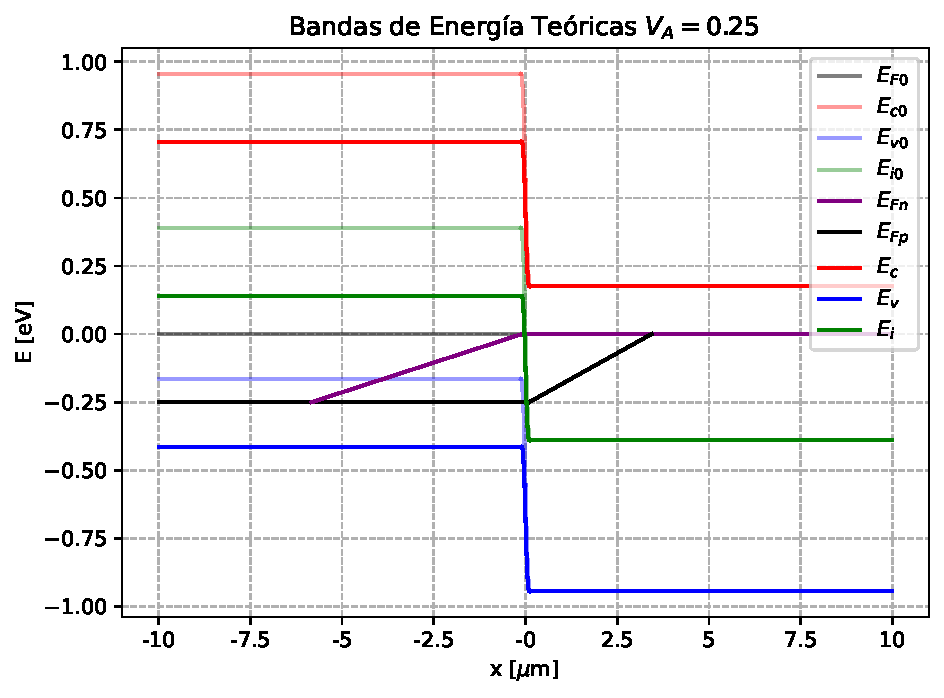
\includegraphics[width=1\linewidth]{Teorico/Bandas_Energia-Directa.pdf}
        \end{figure}
        \vspace{-0.6cm}
        \begin{table}
            \caption{bandas en el equilibrio.}
            \begin{tabular}{c|ccc}
                & \tiny{$E_c$ (P$|$N)} \tiny{[eV]} & \tiny{$E_i$ (P$|$N)} \tiny{[eV]} & \tiny{$E_v$ (P$|$N)} \tiny{[eV]} \\ \hline

                \tiny{Teo.} & \tiny{0.955$|$0.176} & \tiny{0.391$|$-0.391} & \tiny{-0.162$|$-0.944} \\

                \tiny{Sim.} & \tiny{0.956$|$0.176} & \tiny{0.390$|$-0.390} &  \tiny{-0.165$|$-0.944} 
            \end{tabular}
        \end{table}
    \end{column}
    \begin{column}{0.45\textwidth} \begin{center}
        \vspace{-0.55cm}
        \begin{figure} \centering
            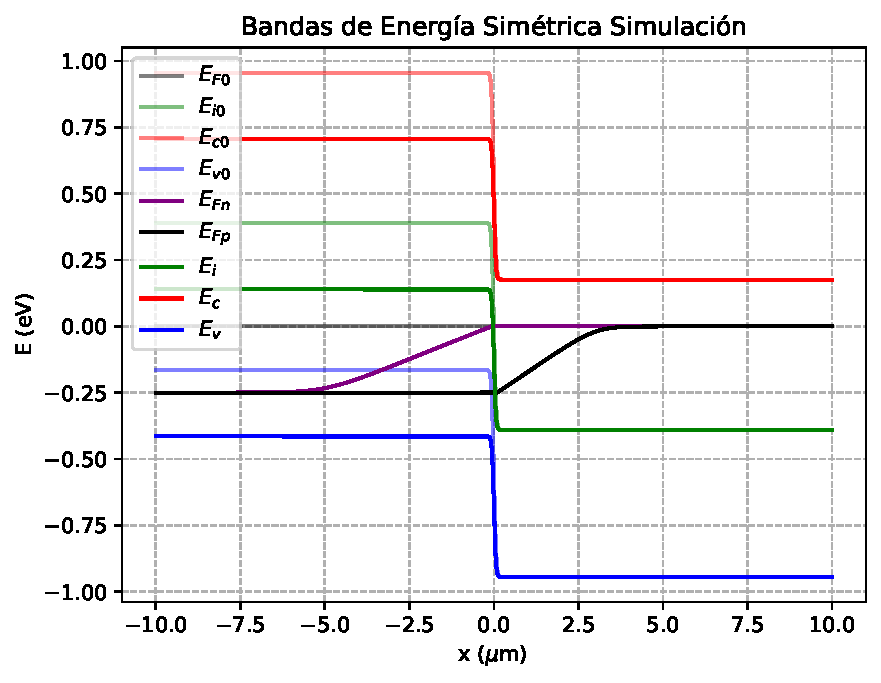
\includegraphics[width=1\linewidth]{Directa/Bandas_Energia-Directa.pdf}
        \end{figure}
        \vspace{-0.35cm}
        \begin{table}
            \caption{bandas en polarización directa.}
            \vspace{-0.48cm}
            \begin{tabular}{c|ccccc}
                & \tiny{$E_c$ (P$|$N)} \tiny{[eV]} & \tiny{$E_i$ (P$|$N)} \tiny{[eV]} & \tiny{$E_v$ (P$|$N)} \tiny{[eV]}  & \tiny{$E_{fp}$ [eV]} (P) & \tiny{$E_{fn}$ [eV]} (N) \\ \hline
    
                \tiny{Teo.} & \tiny{0.705$|$0.176} & \tiny{0.140$|$-0.390} & \tiny{-0.412$|$-0.944} & \tiny{-0.25} & \tiny{0.0} \\
                \tiny{Sim.} & \tiny{0.706$|$0.176} & \tiny{0.140$|$-0.390} & \tiny{-0.414$|$-0.944} & \tiny{-0.25} & \tiny{0.0} \\
            \end{tabular}
        \end{table}
    \end{center}
    \end{column}
    \hspace{2.3cm}
    \end{columns}
\end{frame}


\begin{frame}{Polarización Inversa Diodo No Simétrico: bandas de energía}
    \begin{columns}
    \begin{column}{0.45\textwidth}
        \vspace{-0.55cm}

        \begin{figure}
            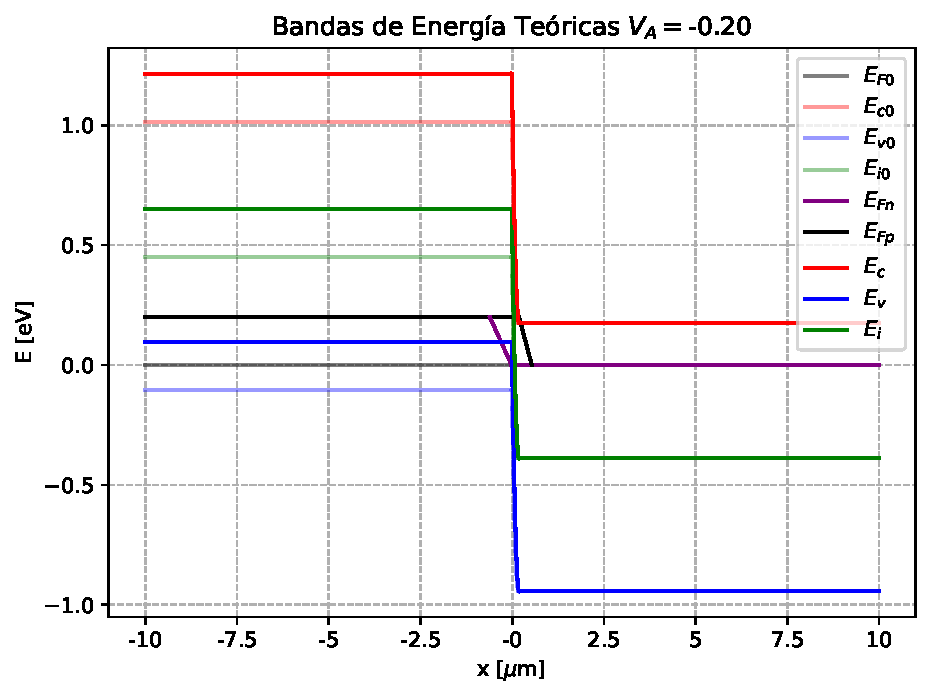
\includegraphics[width=1\linewidth]{Teorico/Bandas_Energia-Inversa.pdf}
        \end{figure}
        \vspace{-0.6cm}
        \begin{table}
            \caption{bandas en el equilibrio.}
            \begin{tabular}{c|ccc}
                & \tiny{$E_c$ (P$|$N)} \tiny{[eV]} & \tiny{$E_i$ (P$|$N)} \tiny{[eV]} & \tiny{$E_v$ (P$|$N)} \tiny{[eV]} \\ \hline

                \tiny{Teo.} & \tiny{1.015$|$0.176} & \tiny{0.449$|$-0.390} & \tiny{-0.105$|$-0.944} \\


                \tiny{Sim.} & \tiny{1.015$|$0.176} & \tiny{0.449$|$-0.390} &  \tiny{-0.105$|$-0.944} 
            \end{tabular}
        \end{table}
    \end{column}
    \begin{column}{0.45\textwidth}
        \vspace{-0.45cm}
        \begin{figure} \centering
            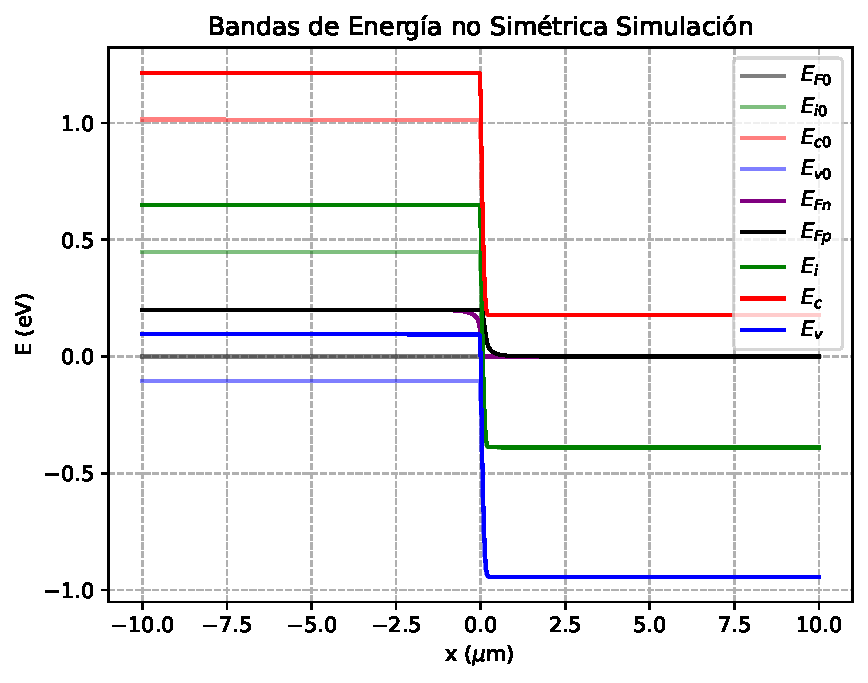
\includegraphics[width=1\linewidth]{Inversa/Bandas_Energia-Inversa.pdf}
        \end{figure}
        \vspace{-0.6cm}
        \begin{table}
            \caption{bandas en polarización inversa.}
            \vspace{-0.7cm}
            \begin{tabular}{c|ccccc}
                & \tiny{$E_c$ (P$|$N)} \tiny{[eV]} & \tiny{$E_i$ (P$|$N)} \tiny{[eV]} & \tiny{$E_v$ (P$|$N)} \tiny{[eV]}  & \tiny{$E_{fp}$ [eV]} (P) & \tiny{$E_{fn}$ [eV]} (N) \\ \hline
    
                \tiny{Teo.} & \tiny{1.215$|$0.176} & \tiny{0.649$|$-0.390} & \tiny{0.095$|$-0.944} & \tiny{0.2} & \tiny{0.0} \\

                \tiny{Sim.} & \tiny{1.215$|$0.176} & \tiny{0.649$|$-0.390} & \tiny{0.095$|$-0.944} & \tiny{0.2} & \tiny{0.0} \\
            \end{tabular}
        \end{table}
    \end{column}
    \hspace{2.3cm}
    \end{columns}
\end{frame}

\begin{frame}{¿Degeneración en las bandas?}
    Como podemos observar \textit{ninguna de las bandas está degenerada}, ya que 

    \begin{equation}
        3kT = 0.078 \ \text{eV}
    \end{equation}
    y tanto $E_c$ como $E_v$ están a una distancia mayor de $E_F$. El valor más cercano se da en la polarización inversa, tanto para $E_v$ en la zona masiva P con una distancai de  $0.105$ eV respecto $E_F$ y para $E_c$ en la zona masiva N con una distancia de 0.176 eV respecto $E_F$.
\end{frame}


\begin{frame}{Polarización directa: campo eléctrico}    \begin{columns}
    \begin{column}{0.5\textwidth}
        \begin{figure}
            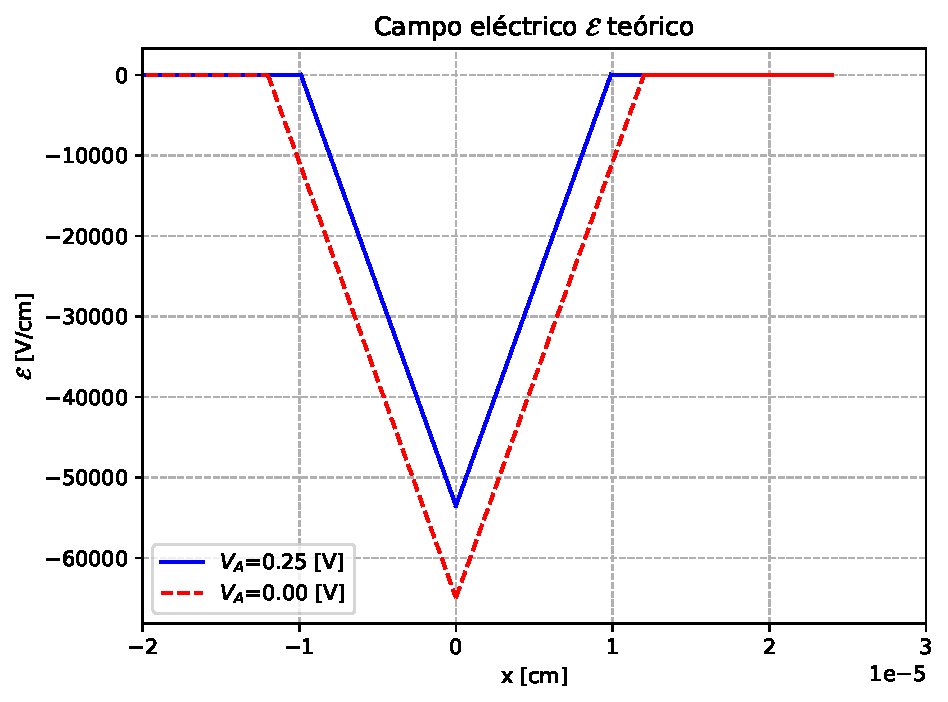
\includegraphics[width=0.90\linewidth]{Teorico/Campo_Electrico-Directa.pdf}
        \end{figure}
    \end{column}
    \begin{column}{0.5\textwidth}
        \begin{figure}
            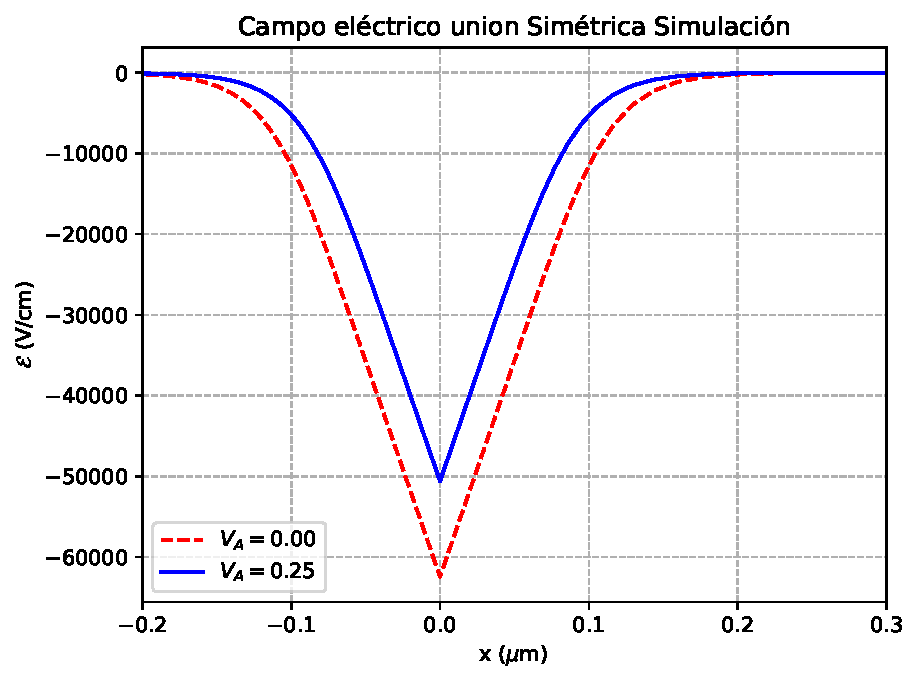
\includegraphics[width=0.90\linewidth]{Directa/Campo_Electrico-Directa.pdf}
        \end{figure}
    \end{column}
    \end{columns}
    \begin{table}
        \caption{Valores del campo eléctrico}
        \begin{tabular}{c|cc}
            & $\mathcal{E}_{\min} (V_A=0)$ [V/cm] & $\mathcal{E}_{\min} (V_A=0.25)$ [V/cm]   \\ \hline
            Teórico & -64940 & -53516 \\
            Simulado & -62474 & -50609
        \end{tabular}
    \end{table}
\end{frame}
\begin{frame}{Polarización inversa: campo eléctrico}
    \begin{columns}
    \begin{column}{0.5\textwidth}
        \begin{figure}
            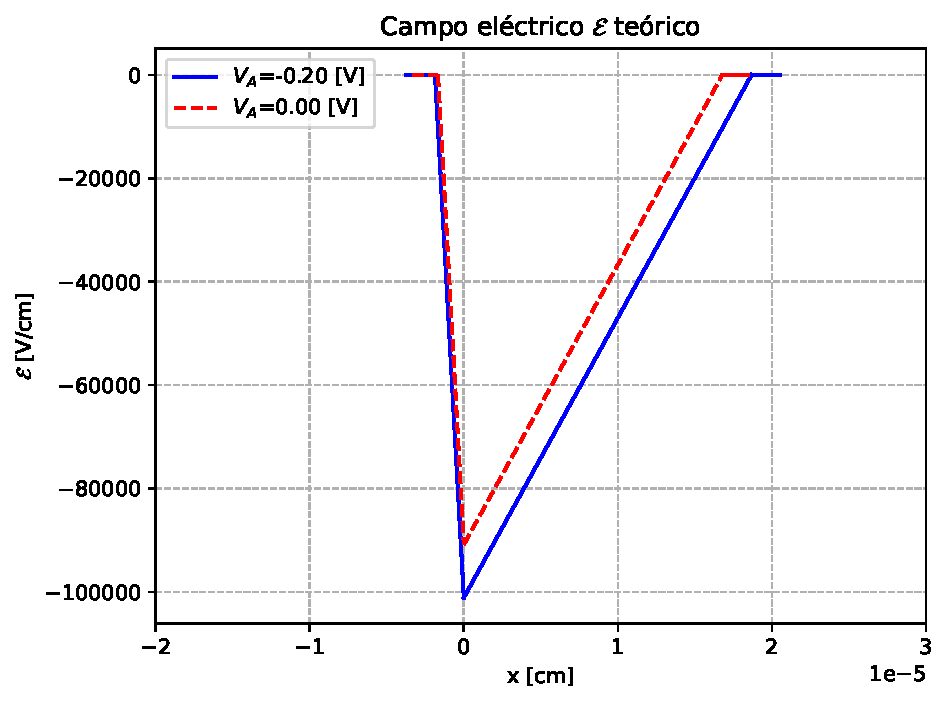
\includegraphics[width=0.90\linewidth]{Teorico/Campo_Electrico-Inversa.pdf}
        \end{figure}
    \end{column}
    \begin{column}{0.5\textwidth}
        \begin{figure}
            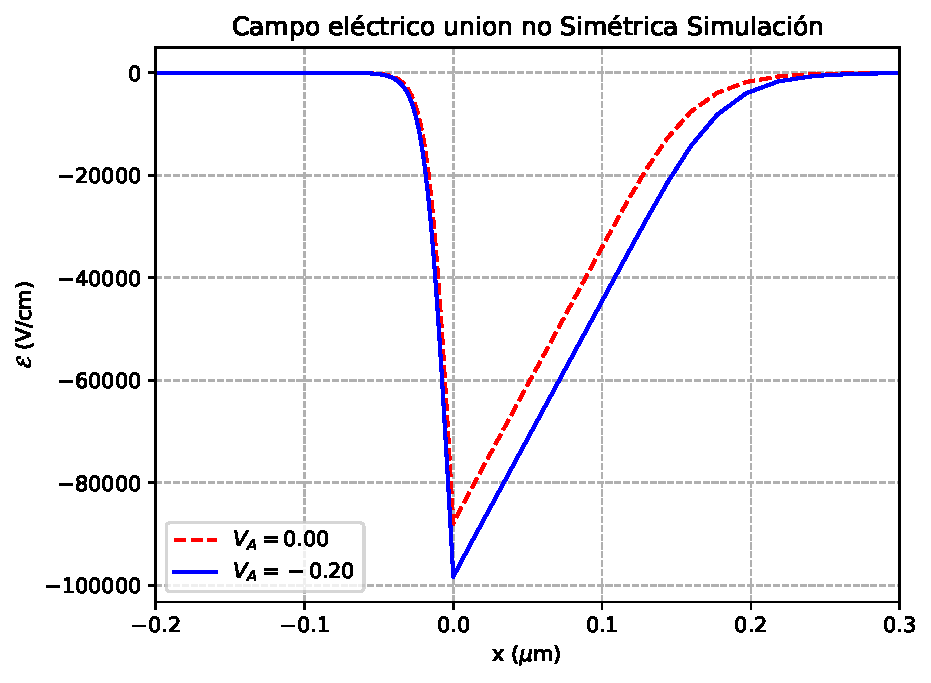
\includegraphics[width=0.90\linewidth]{Inversa/Campo_Electrico-Inversa.pdf}
        \end{figure}
    \end{column}
    \end{columns}
    \begin{table}
        \caption{Valores del campo eléctrico}
        \begin{tabular}{c|cc}
            & $\mathcal{E}_{\min} (V_A=0)$ [V/cm] & $\mathcal{E}_{\min} (V_A=-0.2)$ [V/cm]  \\ \hline
            Teórico & -90849 & -101103 \\
            Simulado & -90463 & -98343 
        \end{tabular}
    \end{table}
\end{frame}

\begin{frame}{Polarización directa: potencial eléctrico}
    
    \begin{columns}
        \begin{column}{0.5\textwidth}
            \begin{figure}
                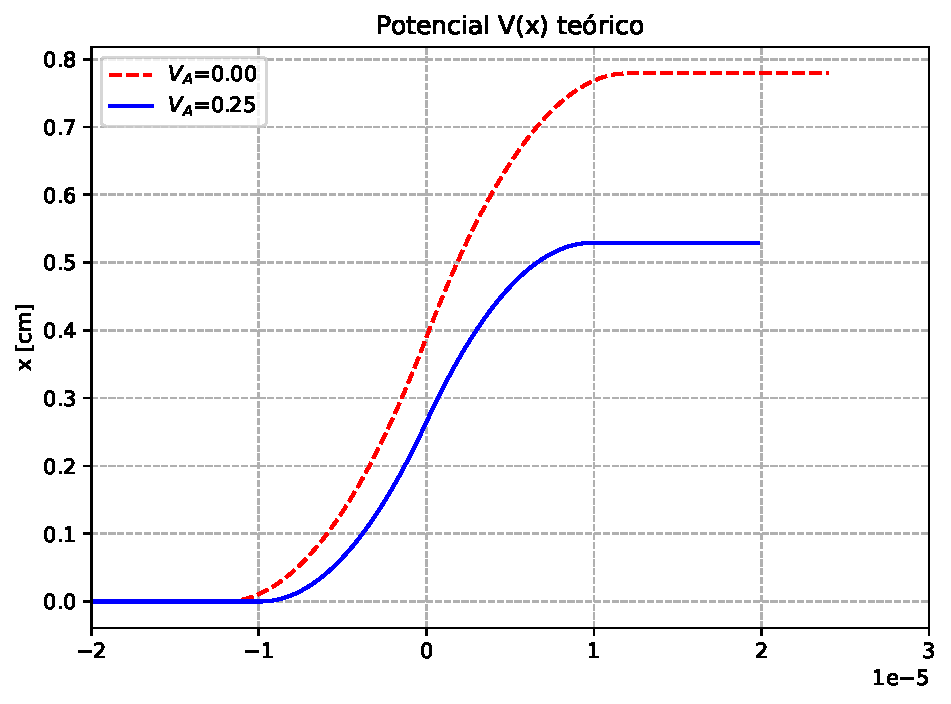
\includegraphics[width=0.90\linewidth]{Teorico/Potencial_Electrico-Directa.pdf}
            \end{figure}
        \end{column}
        \begin{column}{0.5\textwidth}
            \begin{figure}
                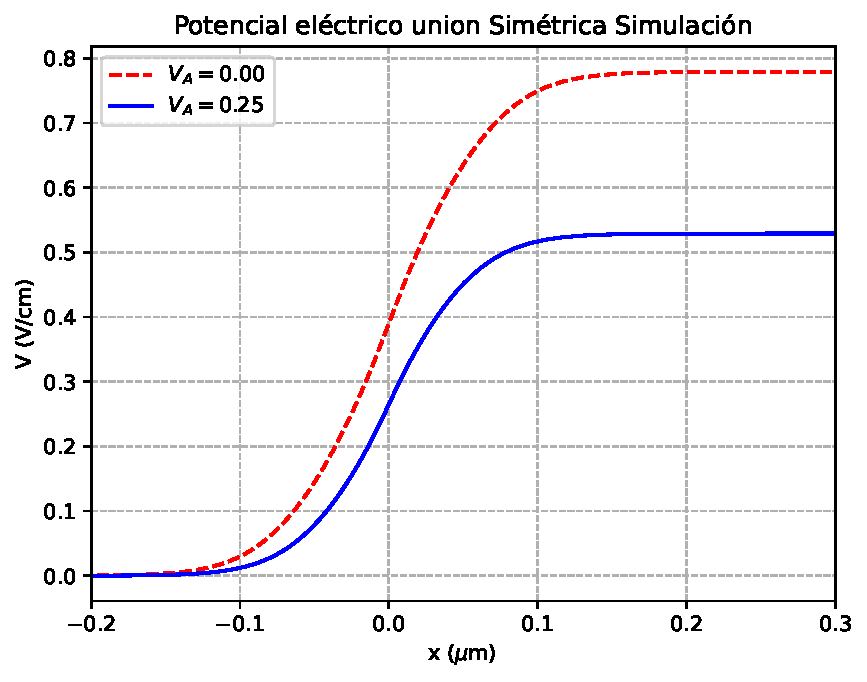
\includegraphics[width=0.90\linewidth]{Directa/Potencial_Electrico-Directa.pdf}
            \end{figure}
        \end{column}
        \end{columns}
        \begin{table}
            \caption{Valores del potencial eléctrico}
            \begin{tabular}{c|cc}
                & $V_J (V_A=0)$ [V] & $V_J (V_A=0.20)$ [V]  \\ \hline
                Teórico & 0.779  & 0.529 \\
                Simulado & 0.779  & 0.530 
            \end{tabular}
        \end{table}
\end{frame}

\begin{frame}{Polarización inversa: potencial eléctrico}
    
    \begin{columns}
        \begin{column}{0.5\textwidth}
            \begin{figure}
                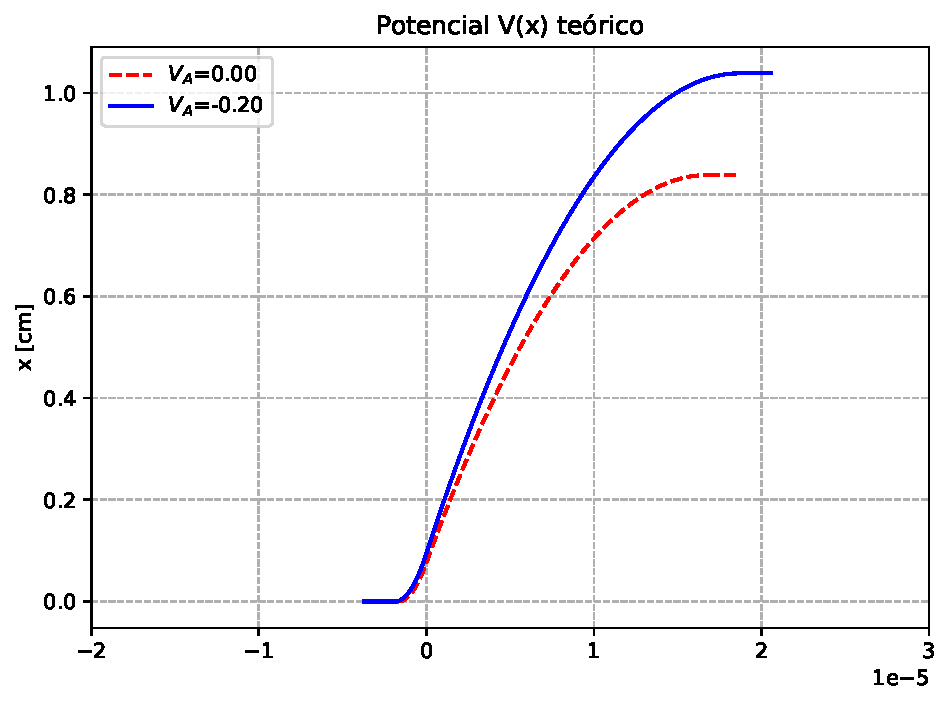
\includegraphics[width=0.90\linewidth]{Teorico/Potencial_Electrico-Inversa.pdf}
            \end{figure}
        \end{column}
        \begin{column}{0.5\textwidth}
            \begin{figure}
                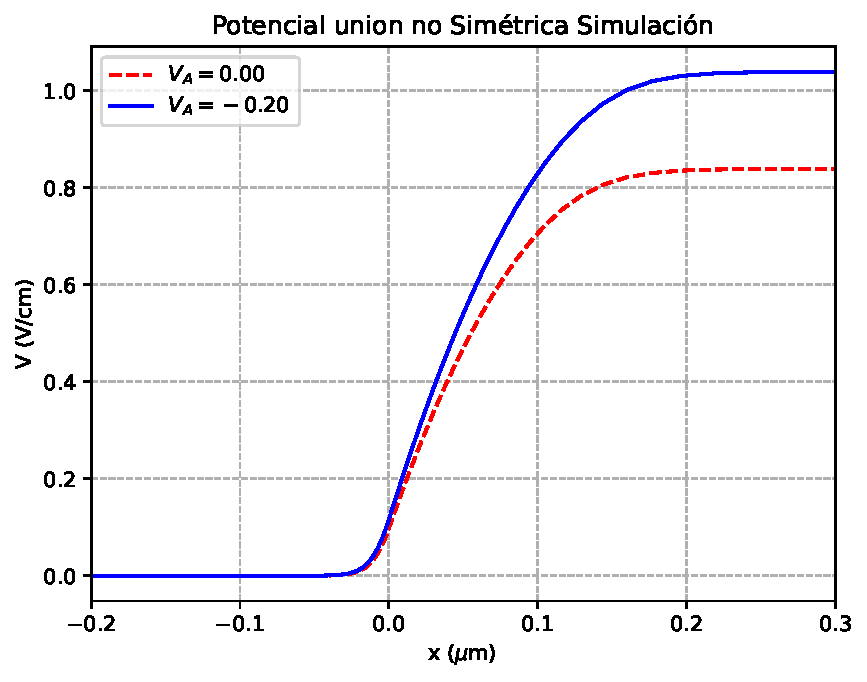
\includegraphics[width=0.90\linewidth]{Inversa/Potencial_Electrico-Inversa.pdf}
            \end{figure}
        \end{column}
        \end{columns}
        \begin{table}
            \caption{Valores del potencial eléctrico}
            \begin{tabular}{c|cc}
                & $V_J (V_A=0)$ [V] & $V_J (V_A=-0.25)$ [V] \\ \hline
                Teórico & 0.839 & 1.039 \\
                Simulado & 0.839 & 1.038 
            \end{tabular}
        \end{table}
\end{frame}

\begin{frame}{Polarización directa: densidad de carga}
    \begin{columns}
        \begin{column}{0.5\textwidth}
            \begin{figure}
                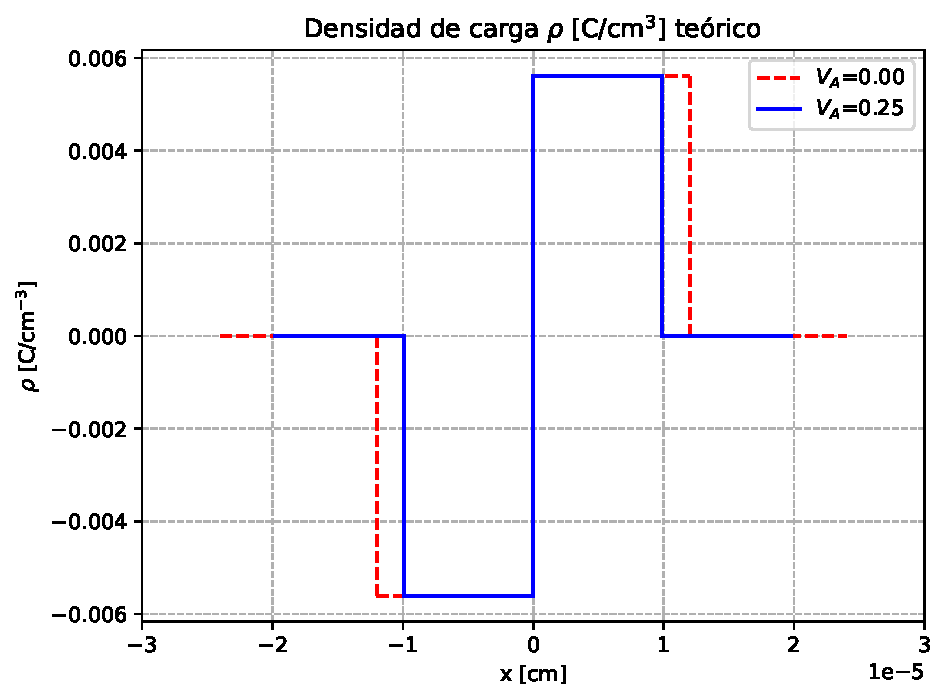
\includegraphics[width=0.90\linewidth]{Teorico/Densidad_Carga-Directa.pdf}
            \end{figure}
        \end{column}
        \begin{column}{0.5\textwidth}
            \begin{figure}
                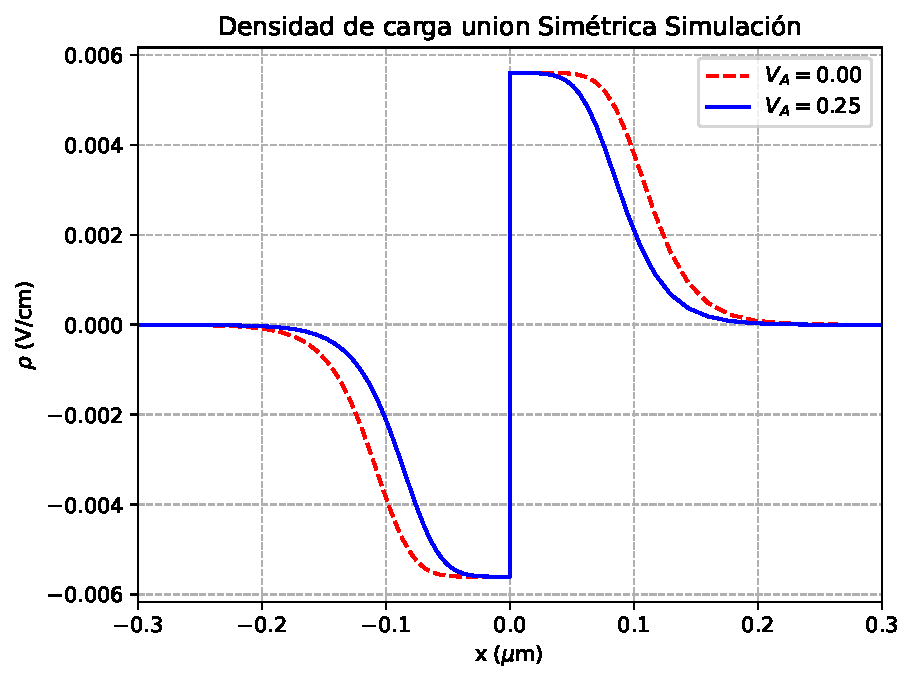
\includegraphics[width=0.90\linewidth]{Directa/Densidad_Carga-Directa.pdf}
            \end{figure}
        \end{column}
        \end{columns}
        \begin{table}
            \caption{Valores de la densidad de carga. El interior indica $V_A$, i.e. $\rho(V_A=0.0)\equiv\rho(0)$. El superíndice máx indica que es el valor máximo de $\rho$.}
            \begin{tabular}{c|cc|cc}
                & $\rho_p^{\max} (0)$ \tiny{[C/cm$^{3}$]} & $\rho_p^{\max} (0.2)$ \tiny{[C/cm$^{3}$]}  & $\rho_n^{\max} (0)$ \tiny{[C/cm$^{3}$]}  & $\rho_n ^{\max} (0.2)$ \tiny{[C/cm$^{3}$]}  \\ \hline
                Teórico &  -0.00561 &- 0.00561 & 0.00561 & 0.00561 \\
                Simulado & -0.00561 & -0.00561 &  0.0561 & 0.0561
            \end{tabular}
        \end{table}
\end{frame}

\begin{frame}{Polarización inversa: densidad de carga}
    \begin{columns}
        \begin{column}{0.5\textwidth}
            \begin{figure}
                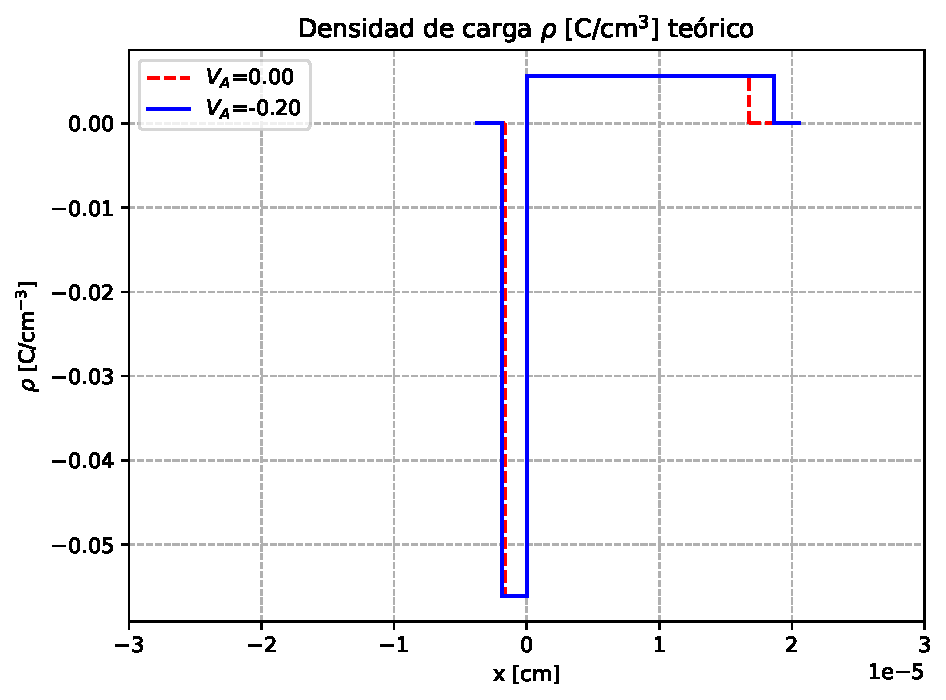
\includegraphics[width=0.90\linewidth]{Teorico/Densidad_Carga-Inversa.pdf}
            \end{figure}
        \end{column}
        \begin{column}{0.5\textwidth}
            \begin{figure}
                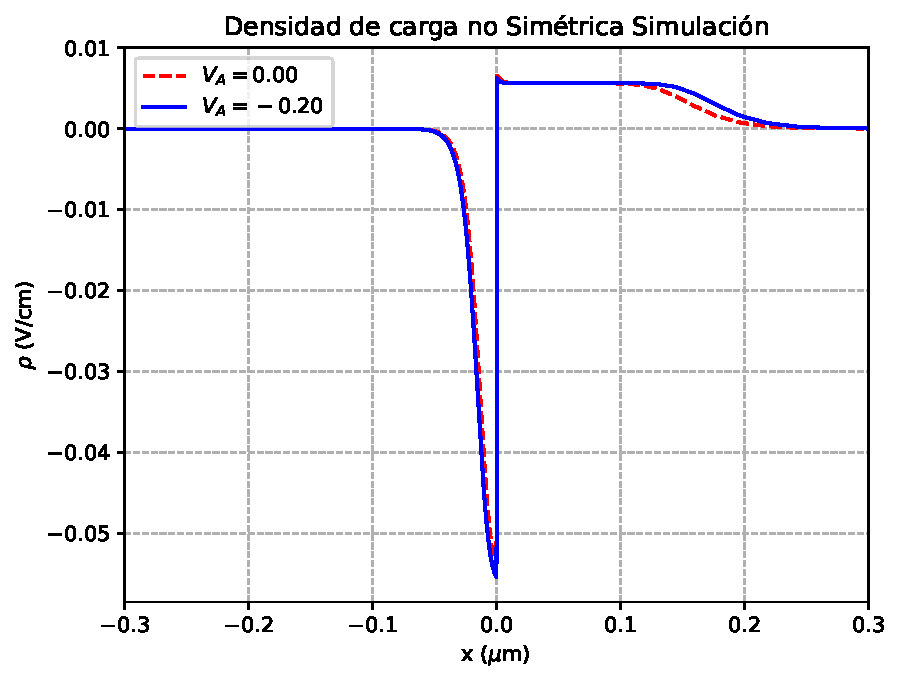
\includegraphics[width=0.90\linewidth]{Inversa/Densidad_Carga-Inversa.pdf}
            \end{figure}
        \end{column}
        \end{columns}
        \begin{table}
            \caption{Valores de la densidad de carga. El interior indica $V_A$, i.e. $\rho(V_A=0.0)\equiv\rho(0)$. El superíndice máx indica que es el valor máximo de $\rho$.}
            \begin{tabular}{c|cc|cc}
                & $\rho_p^{\max} (0)$ \tiny{[C/cm$^3$]} & $\rho_p^{\max} (0.2)$ \tiny{[C/cm$^{3}$]}  & $\rho_n^{\max} (0)$ \tiny{[C/cm$^{3}$]}  & $\rho_n ^{\max} (0.2)$ \tiny{[C/cm$^{3}$]}  \\ \hline
                Teórico & -0.0561 & -0.0561 & 0.00561 & 0.00561 \\
                Simulado & -0.05466 & -0.05537  & 0.00690 &  0.00630
            \end{tabular}
        \end{table}

\end{frame}

\begin{frame}{Polarización directa: portadores minoritarios}
    \begin{columns}
        \begin{column}{0.5\textwidth}
            \begin{figure}
                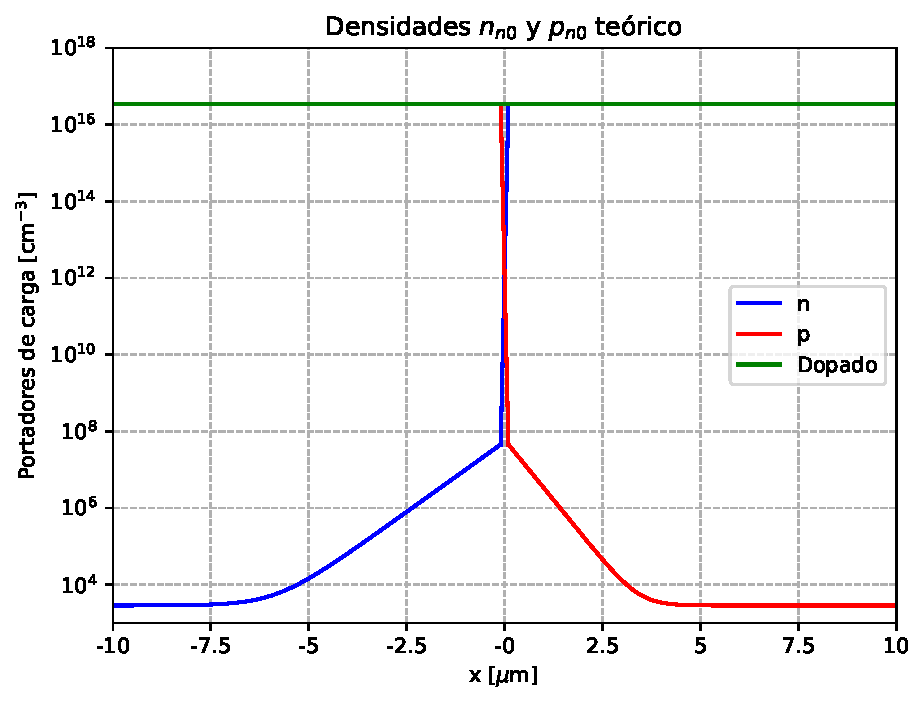
\includegraphics[width=0.90\linewidth]{Teorico/Bandas_Minoritarios-Directa.pdf}
            \end{figure}
        \end{column}
        \begin{column}{0.5\textwidth}
            \begin{figure}
                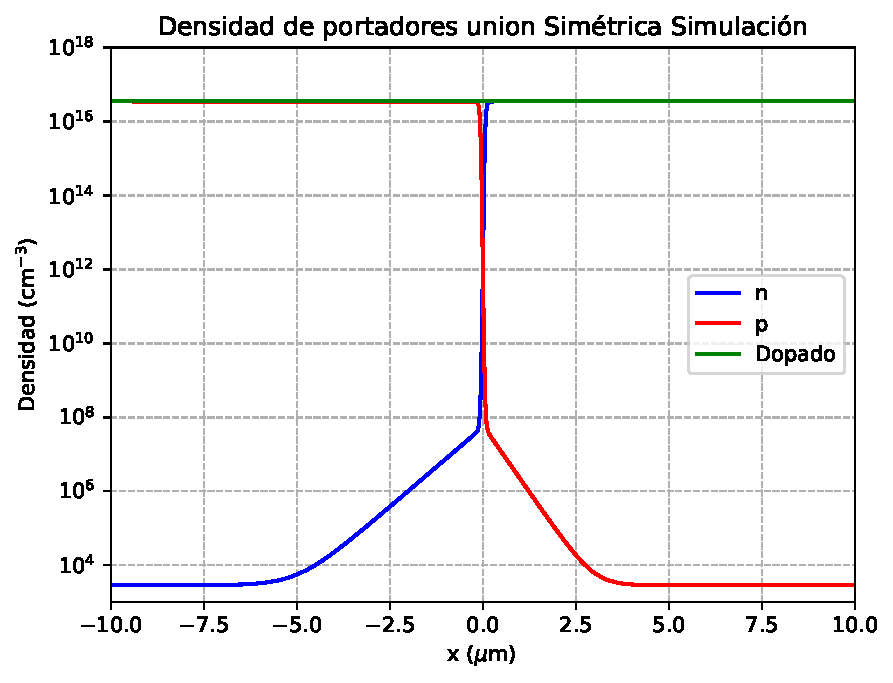
\includegraphics[width=0.90\linewidth]{Directa/Bandas_Minoritarios-Directa.pdf}
            \end{figure}
        \end{column}
        \end{columns}
        \begin{table}
            \caption{Valores de los portadores minoritarios. Los $\Delta n_p$ y $\Delta p_n$ los evaluamos en $x_n$ y $x_p$ obtenidos usando las bandas de energías (simuladas).}
            \begin{tabular}{c|cccc}
                & $n_{p0} $  \tiny{[cm$^{-3}$]}  & $\Delta n_p$ \tiny{[cm$^{-3}$]}  & $p_{n0}$ \tiny{[cm$^{-3}$]}  & $\Delta p_n$  \tiny{[cm$^{-3}$]}  \\ \hline
                Teórico & 2857 & 4.53$\cdot 10^7$  & 2857 & 4.53$\cdot 10^7$ \\
                Simulado & 2835 & 4.72$\cdot 10^7$ & 2835 & 4.44$\cdot 10^7$
            \end{tabular}
        \end{table}
\end{frame}

\begin{frame}{Polarización directa: portadores minoritarios}
    \begin{columns}
        \begin{column}{0.5\textwidth}
            \begin{figure}
                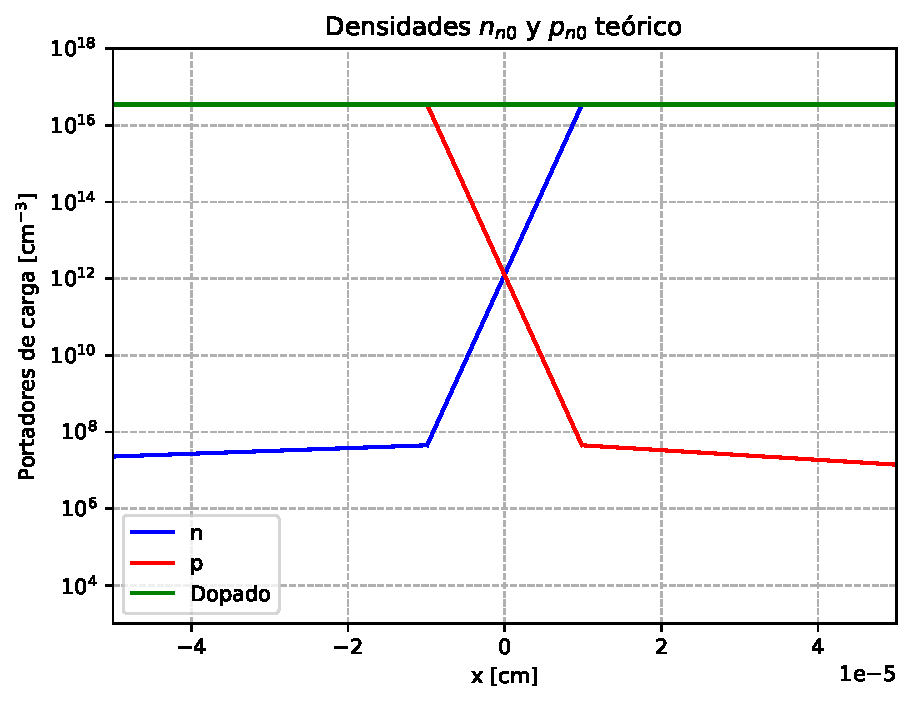
\includegraphics[width=0.90\linewidth]{Teorico/Densidad_portadores_directa_cortada.pdf}
            \end{figure}
        \end{column}
        \begin{column}{0.5\textwidth}
            \begin{figure}
                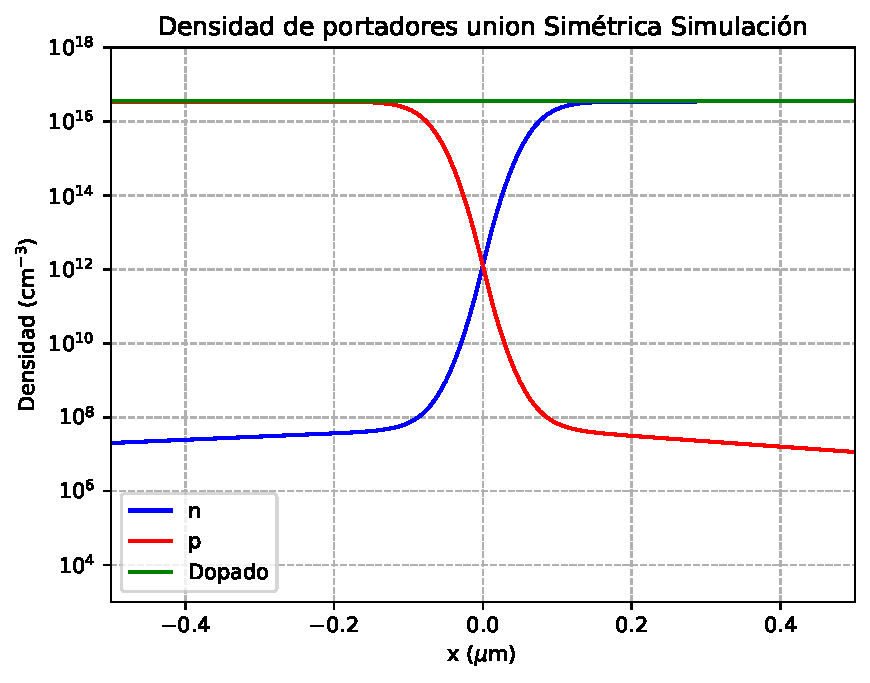
\includegraphics[width=0.90\linewidth]{Directa/Densidad_portadores_directa_cortada.pdf}
            \end{figure}
        \end{column}
        \end{columns}
        Cabe destacar que para el cálculo de las 
\end{frame}



\begin{frame}{Polarización inversa: portadores minoritarios}
    
    \begin{columns}
        \begin{column}{0.5\textwidth}
            \begin{figure}
                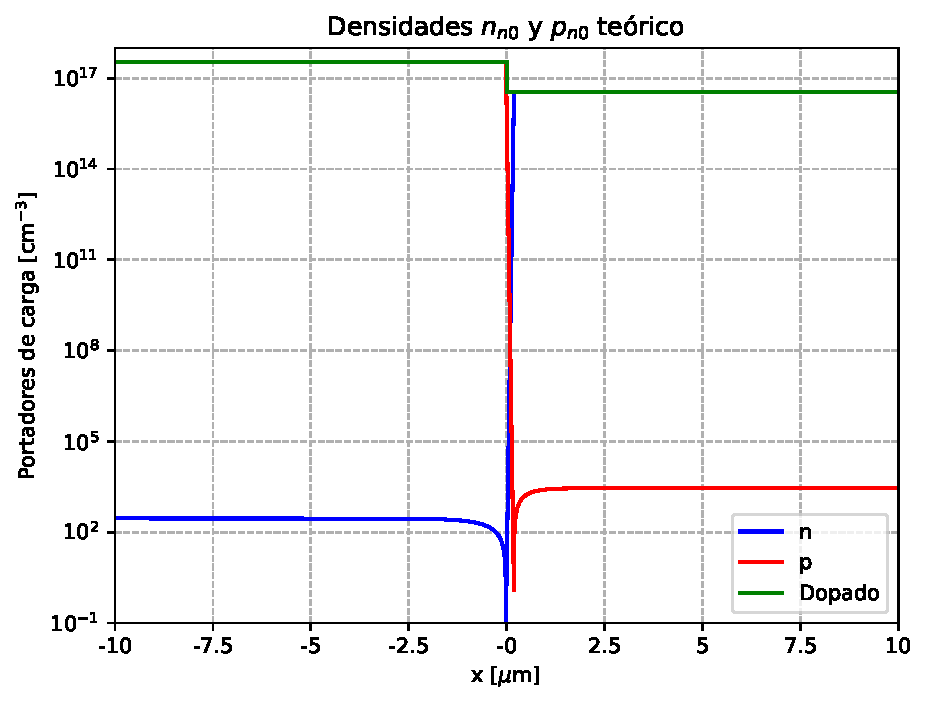
\includegraphics[width=0.90\linewidth]{Teorico/Bandas_Minoritarios-Inversa.pdf}
            \end{figure}
        \end{column}
        \begin{column}{0.5\textwidth}
            \begin{figure}
                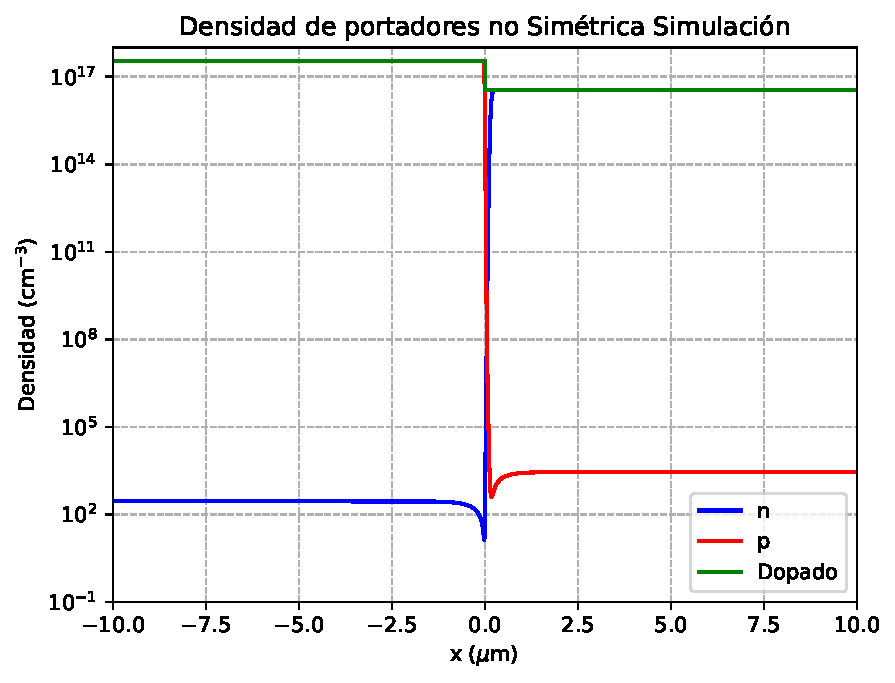
\includegraphics[width=0.90\linewidth]{Inversa/Bandas_Minoritarios-Inversa.pdf}
            \end{figure}
        \end{column}
        \end{columns}
        \begin{table}
            \caption{Valores de los portadores minoritarios. Los $\Delta n_p$ y $\Delta p_n$ los evaluamos en $x_n$ y $x_p$ obtenidos usando las bandas de energías (simuladas).}
            \begin{tabular}{c|cccc}
                & $n_{p0} $ \tiny{[cm$^{-3}$]} & $\Delta n_p$ \tiny{[cm$^{-3}$]}  & $p_{n0} $  \tiny{[cm$^{-3}$]}  & $\Delta p_n$ \tiny{[cm$^{-3}$]}   \\ \hline
                Teórico & 2857 & -285.59  & 2857 & 2855.9 \\
                Simulado & 283.58 & -270.17 & 2835  & -2393 
            \end{tabular}
        \end{table}
\end{frame}

\begin{frame}{Polarización inversa: portadores minoritarios}
        \begin{columns}
            \begin{column}{0.5\textwidth}
                \begin{figure}
                    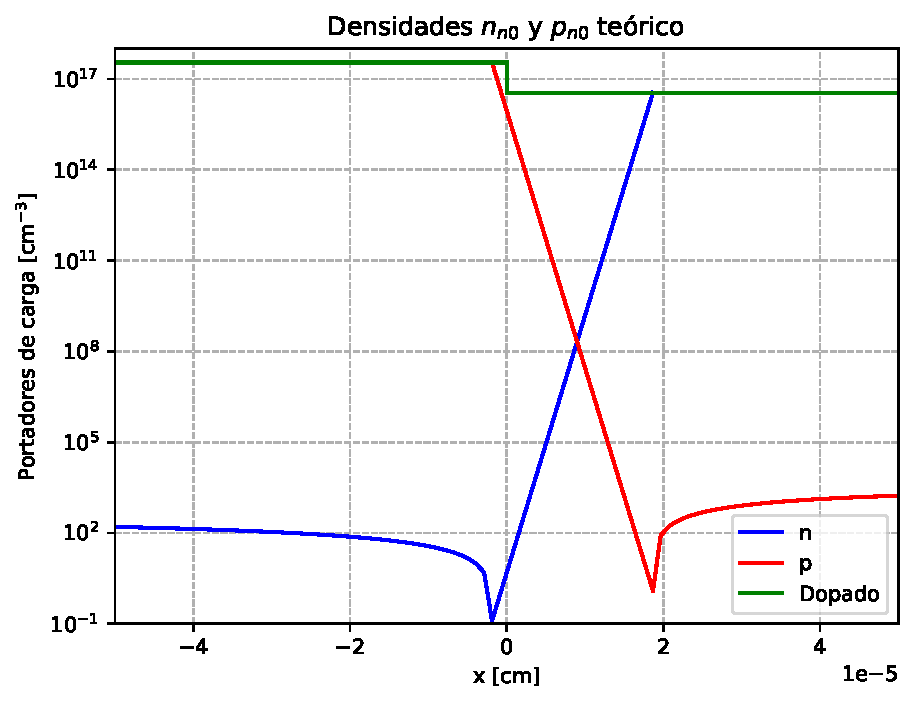
\includegraphics[width=0.90\linewidth]{Teorico/Densidad_portadores_inversa_cortada.pdf}
                \end{figure}
            \end{column}
            \begin{column}{0.5\textwidth}
                \begin{figure}
                    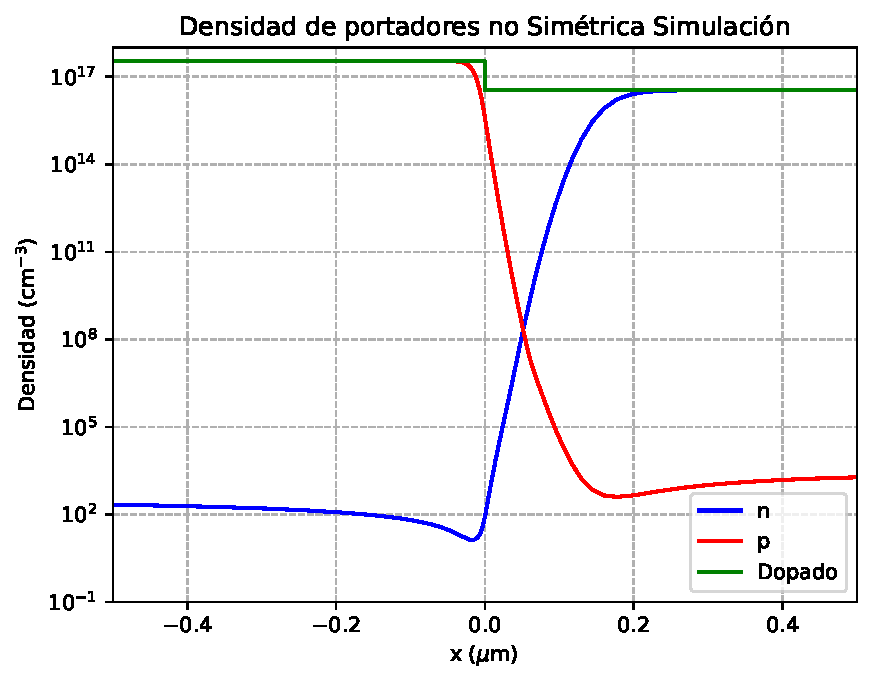
\includegraphics[width=0.90\linewidth]{Inversa/Densidad_portadores_inversa_cortada.pdf}
                \end{figure}
            \end{column}
        \end{columns}
\end{frame}



\begin{frame}{Curva I-V: directa}
    \begin{columns}
        \begin{column}{0.5\textwidth}
            \begin{figure}
                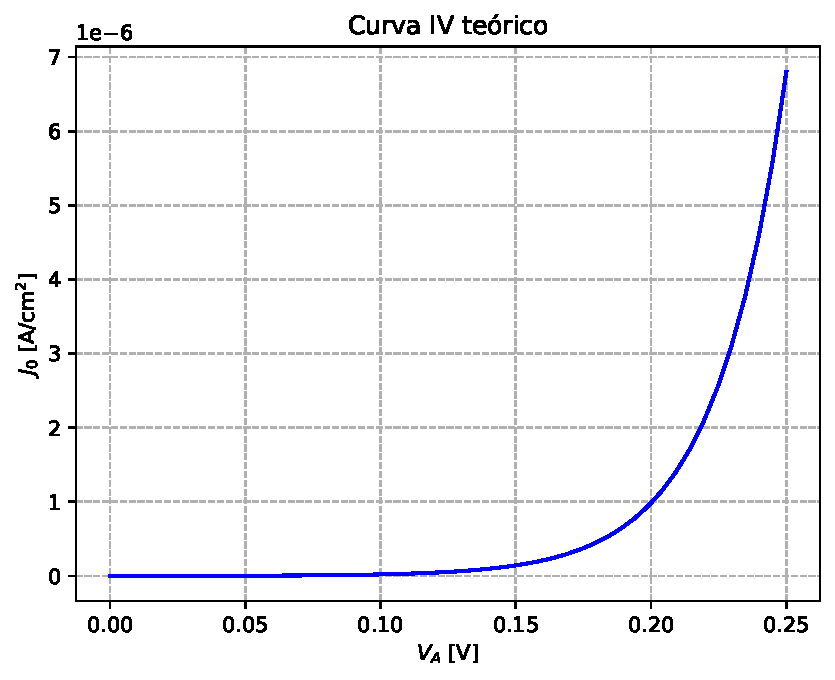
\includegraphics[width=0.90\linewidth]{Teorico/Intensidades-Directa.pdf}
            \end{figure}
        \end{column}
        \begin{column}{0.5\textwidth}
            \begin{figure}
                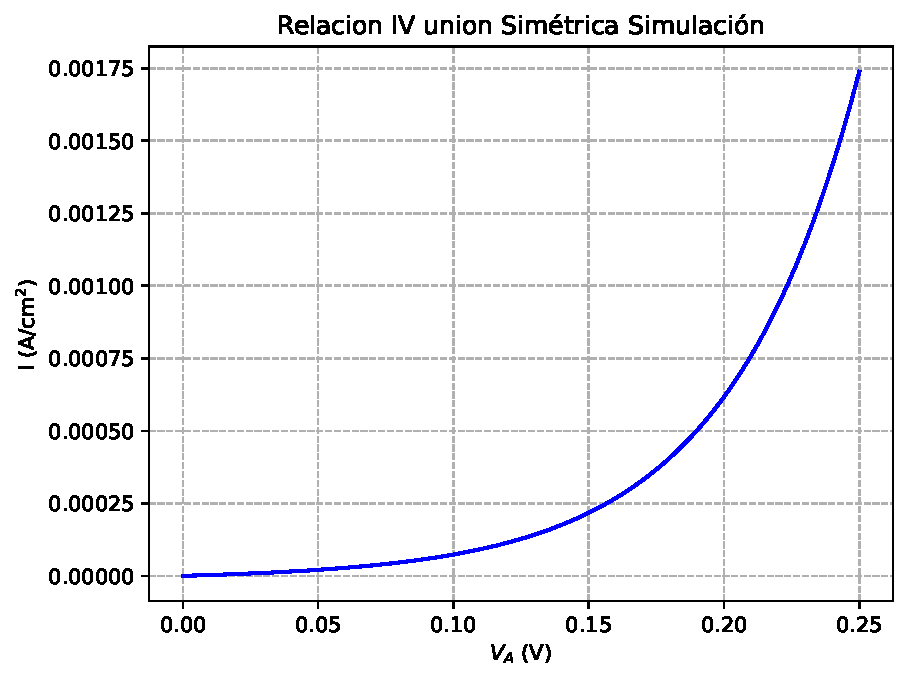
\includegraphics[width=0.90\linewidth]{Directa/Intensidades-Directa.pdf}
            \end{figure}
        \end{column}
        \end{columns}
        \begin{table}
            \caption{Valores de las intensidades}
            \begin{tabular}{c|c}
                  & $I(V_A=0.25)$ \tiny{[A/cm$^2$]}  \\ \hline
                Teórico & 6.80$\cdot 10^{-6}$ \\
                Simulado & 1.74$\cdot 10^{-3}$
            \end{tabular}
        \end{table}
\end{frame}

\begin{frame}{Curva I-V: inversa}
    \begin{columns}
        \begin{column}{0.5\textwidth}
            \begin{figure}
                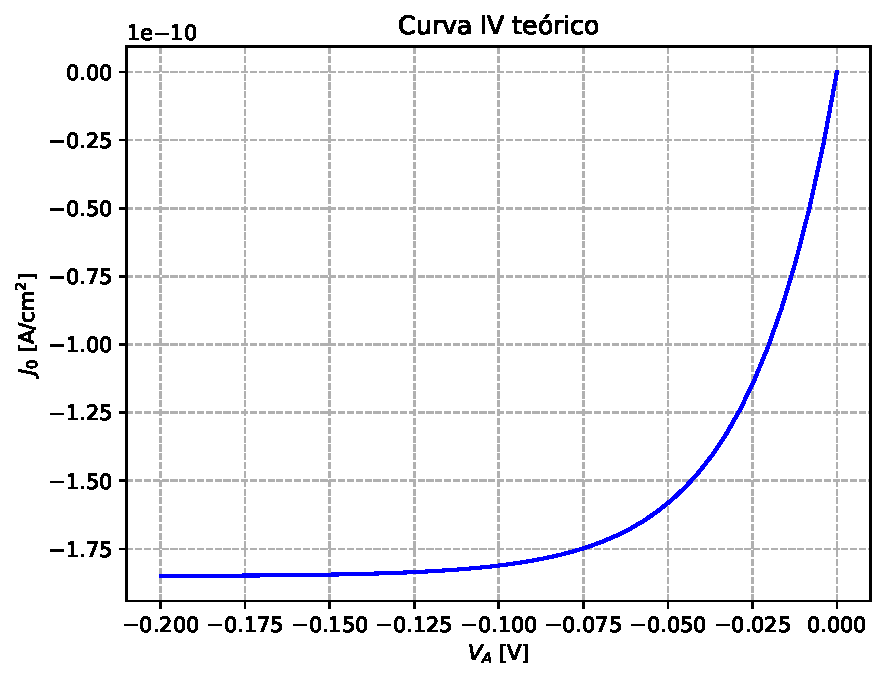
\includegraphics[width=0.90\linewidth]{Teorico/Intensidades-Inversa.pdf}
            \end{figure}
        \end{column}
        \begin{column}{0.5\textwidth}
            \begin{figure}
                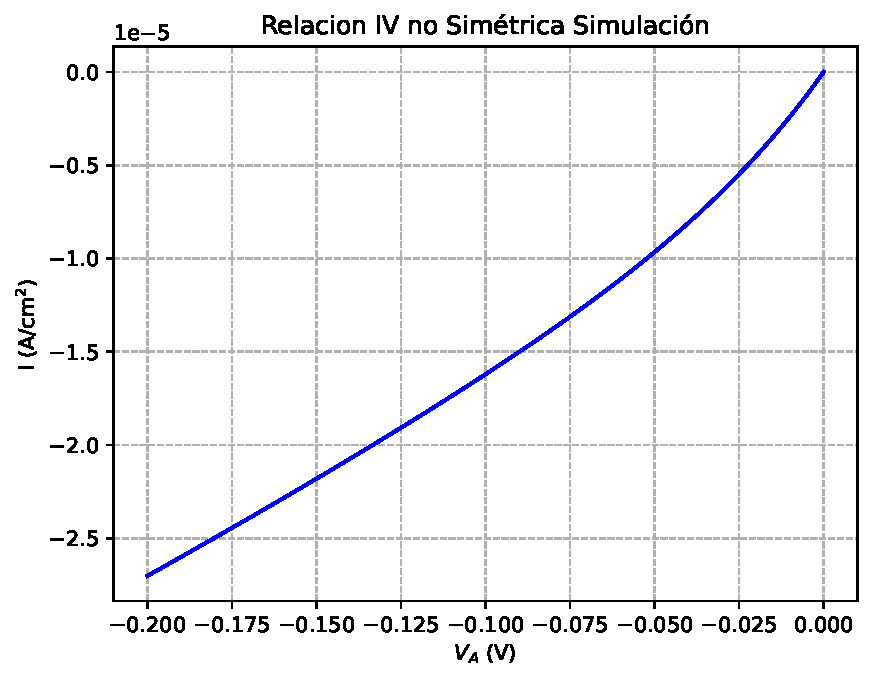
\includegraphics[width=0.90\linewidth]{Inversa/Intensidades-Inversa.pdf}
            \end{figure}
        \end{column}
        \end{columns}
        \begin{table}
            \caption{Valores de las intensidades}
            \begin{tabular}{c|c}
                & $I(V_A=-0.25)$ \tiny{[A/cm$^2$]} \\ \hline
                Teórico &  -1.85 $\cdot 10^{-10}$  \\
                Simulado & -2.70$10^{-5}$  
            \end{tabular}
        \end{table}
\end{frame}

\begin{frame}{Otros valores obtenibles}
    Otros valores que podríamos calcular/obtener con los valores de la simulación podrían ser: $x_n$,$x_p$,$I_0$,$L_N$,$L_P$. Para obtenerlos bastaría con hacer algún tipo de regresión. \\
    \begin{itemize}

    \item Por ejemplo, $x_n$ y $x_p$ podríamos obtenero realizando regresiones lineales en las regiones lineles de $\Ecal(x)$ y viendo en que punto se corta, o por ejemplo ver en que punto comienza a crecer $V(x)$ o $\rho(x)$. 

    \item Otros como $I_0$ serían un poco más difícil de calcular, ya que el comportamiento ideal de IV no es tan preciso, mientras que $L_N$ y $L_P$ sí (a partir de $n_{p0}(x)$ y $p{n0}$). \\

    \end{itemize}

    Sin embargo esto excede los objetivos de esta presentación.
\end{frame}

\section{Conclusiones}

\begin{frame}{Conclusiones}
    Las conclusiones son:     
    \begin{itemize}
        \item El diodo ideal predice el orden de todos los resultados (con una diferencia relativa de entre el $10\%$ y menos del $1\%$), salvo la relación IV en el que falla varios órdendes de magnitud.
        \item En casos particulares como bandas de energías y voltaje máximo la diferencia es mínima.
        \item Las funciones analíticas que se observan del diodo ideal devuelven valores similares a los que da la simulación.
        \item Las principales diferncias entre modelo y simulación se da en los bordes de la región de vaciamiento.
    \end{itemize}
    Con todo, hemos podido observar que para los voltajes de polarización y dopantes dados, el diodo ideal es una buena aproximación (con un margen de error del $10\%$) del diodo PN, excepto para la relación $IV$. 
\end{frame}


%------------------------------------------------o 

%\begin{frame}{References}
%    \footnotesize
%    \bibliography{reference.bib}
%    \bibliographystyle{apalike}
%\end{frame}

%------------------------------------------------

\begin{frame}
    \Huge{\centerline{\textbf{Fin}}}
\end{frame}

%----------------------------------------------------------------------------------------

\end{document}